El Sprint realizado entre el 12/04/2016 y el 04/05/2016 se completó exitosamente. Todas las user stories planificadas fueron terminadas.
A continuación presentamos los burndown charts asociados y el detalle de horas consumidas:

\begin{figure}[h!]
 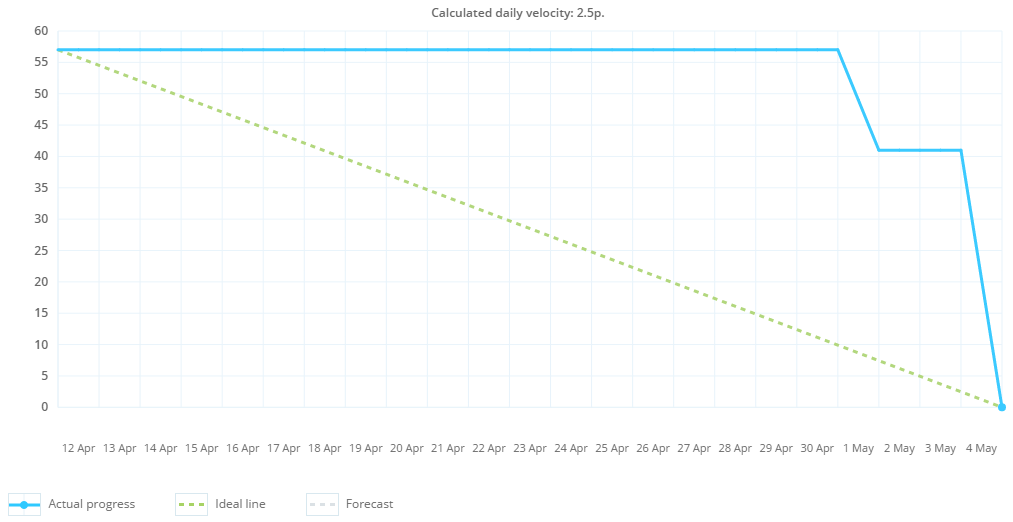
\includegraphics[width=\textwidth]{imagenes/burndown-points.png}
 \caption{Burndonw Chart de Story Points. La línea verde punteada indica el progreso ideal (comienza en 57 puntos, el total de la estimación de esfuerzo).
 La línea azul indica el progreso real.}
\end{figure}

\begin{figure}[h!]
 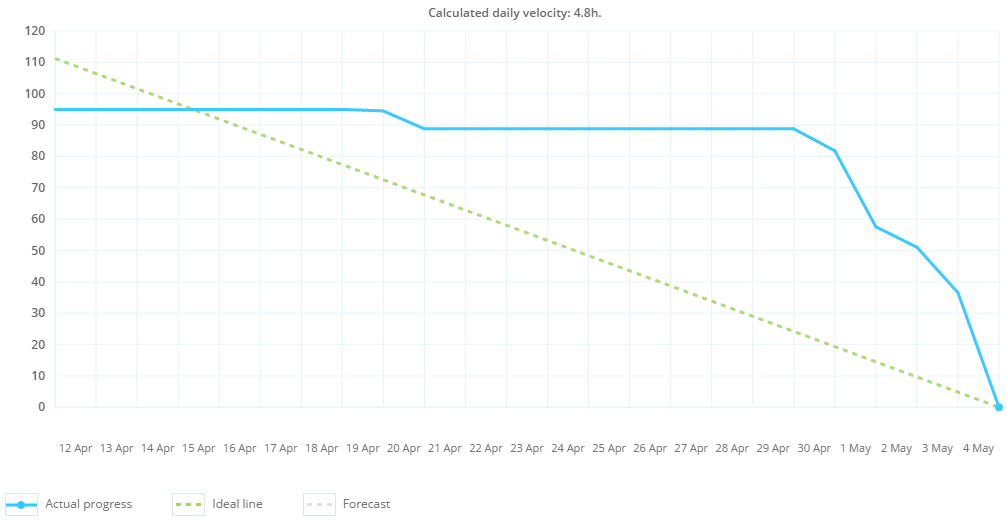
\includegraphics[width=\textwidth]{imagenes/burndown-hours.png}
 \caption{Burndonw Chart de Horas de Tareas. La línea verde punteada indica el progreso ideal (comienza en 111 horas, lo cual difiere de la estimación
 inicial de 96 horas porque se agregaron horas durante el sprint). La línea azul indica el progreso real.}
\end{figure}

En los gráficos se observa que hasta el 19/04 no hubo avance. El 20/04 se realizaron algunas tareas para discutir en la reunión con el Product Owner del
21/04. Hasta aquí no se cerró ninguna story (por eso los Story Points se mantienen constantes). En este momento se detectaron fallas en la estimación
y se agregaron horas a las tareas (es por esto que la horas empiezan estando por debajo del total de horas).

Luego hubo otro período sin avances y finalmente
a partir del 30/04 empezó a haber avance contínuo en las tareas. El 1/05 se cerró la primer user story y de ahí en más se fueron cerrando el resto.

Finalmente, la cantidad de horas hombre consumidas fue de:

\vspace{0.3cm}
\begin{tabular}{ | c | c | }
 \hline
 Horas Integrante 1: & 21\\
 \hline
 Horas Integrante 2: & 14\\
 \hline
 Horas Integrante 3: & 33.5\\
 \hline
 Horas Integrante 4: & 29.5\\
 \hline
 {\bf Horas Totales:} & 92.5\\
 \hline
\end{tabular}

